% ============================================================
% 书脊 (Spine) - Page 3
% 严格按照哈尔滨工程大学模板格式，带黑色竖框
% ============================================================
\newpage
\thispagestyle{empty}

% 页面设置 - 书脊页面
\vspace*{2cm}

% 书脊标签（左上角）
\noindent
\hspace*{2cm}
{\fontsize{12pt}{18pt}\selectfont 书脊}

\vspace{1cm}

% 使用TikZ绘制带黑色竖框的书脊
\begin{center}
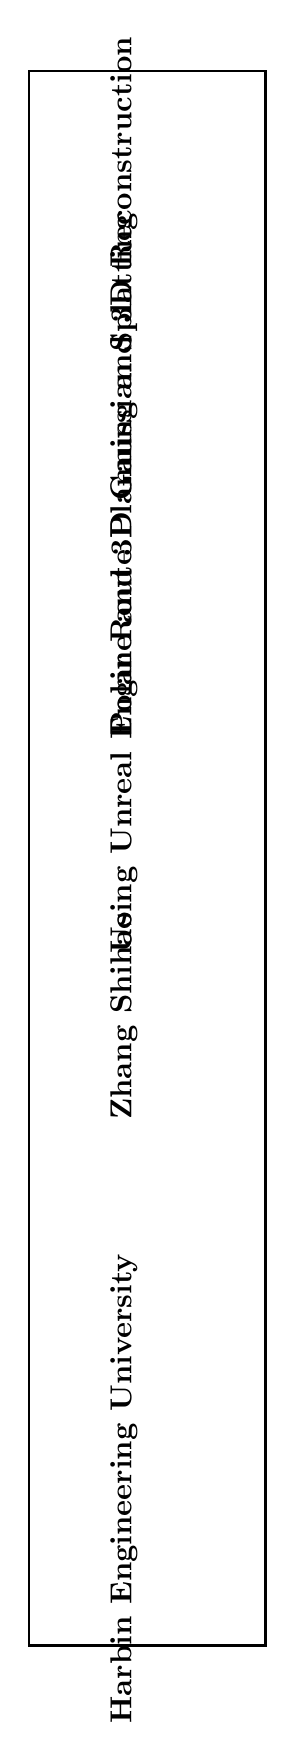
\begin{tikzpicture}
    % 定义书脊框的尺寸和位置
    % 竖框：高度约20cm，宽度约3cm，线宽1pt黑色边框
    \draw[line width=1pt, black]
        (-1.5, -10) rectangle (1.5, 10);

    % 书脊文字内容 - 竖排从下到上（旋转-90度后从上到下）
    % 论文题目
    \node[rotate=90, anchor=south, font=\fontsize{10.5pt}{16pt}\selectfont] at (0, 6) {
        \textbf{Polar Route Planning and 3D Reconstruction}
    };
    \node[rotate=90, anchor=south, font=\fontsize{10.5pt}{16pt}\selectfont] at (0, 3.5) {
        \textbf{Using Unreal Engine and 3D Gaussian Splatting}
    };

    % 分隔空间
    \node[rotate=90, anchor=south] at (0, 1) {};

    % 作者姓名
    \node[rotate=90, anchor=south, font=\fontsize{10.5pt}{16pt}\selectfont] at (0, -2) {
        \textbf{Zhang Shihao}
    };

    % 分隔空间
    \node[rotate=90, anchor=south] at (0, -5) {};

    % 学校名称
    \node[rotate=90, anchor=south, font=\fontsize{10.5pt}{16pt}\selectfont] at (0, -8) {
        \textbf{Harbin Engineering University}
    };
\end{tikzpicture}
\end{center}

\clearpage
